%%%%%%%%%%%%%%%%%%%%%%%%%%%%%%%%%%%%%%%%%%%%%%%%%%%%%%%%%%%%%%%%%%%%%%
%%%%%%%%%%%%%%%%%%%%%%%%%%%%%%%%%%%%%%%%%%%%%%%%%%%%%%%%%%%%%%%%%%%%%%
%%
%% IVT LaTeX template
%%   Kirill Müller
%%   kirill.mueller@ivt.baug.ethz.ch
%%
%%%%%%%%%%%%%%%%%%%%%%%%%%%%%%%%%%%%%%%%%%%%%%%%%%%%%%%%%%%%%%%%%%%%%%
%%%%%%%%%%%%%%%%%%%%%%%%%%%%%%%%%%%%%%%%%%%%%%%%%%%%%%%%%%%%%%%%%%%%%%

%%%%%%%%%%%%%%%%%%%%%%%%%%%%%%%%%%%%%%%%%%%%%%%%%%%%%%%%%%%%%%%%%%%%%%
%%%%%%%%%%%%%%%%%%%%%%%%%%%%%%%%%%%%%%%%%%%%%%%%%%%%%%%%%%%%%%%%%%%%%%
%%
%% Encoding check:
%%   ä  ö  ü  Ä  Ö  Ü  ß  á  é  í  ó  ú  à  è  ì  ò  ù  â  ê  î  ô  û
%%
%%   If the above contains rubbish, please re-open this file using
%%   the CORRECT encoding.  By default this is UTF-8.
%%   DO NOT save the file in this case!
%%
%%%%%%%%%%%%%%%%%%%%%%%%%%%%%%%%%%%%%%%%%%%%%%%%%%%%%%%%%%%%%%%%%%%%%%
%%%%%%%%%%%%%%%%%%%%%%%%%%%%%%%%%%%%%%%%%%%%%%%%%%%%%%%%%%%%%%%%%%%%%%


%%%%%%%%%%%%%%%%%%%%%%%%%%%%%%%%%%%%%%%%%%%%%%%%%%%%%%%%%%%%%%%%%%%%%%
%%%%%%%%%%%%%%%%%%%%%%%%%%%%%%%%%%%%%%%%%%%%%%%%%%%%%%%%%%%%%%%%%%%%%%
%%
%% This is an example for writing a paper at the IVT.
%% It supports English and German language.
%% By using it, it is possible to switch paper layouts easily
%% (e.g., working paper style into TRB style)
%%
%% The easiest way to write you own paper is to create an
%% appropriate directory stucture in the papers subdirectory
%% i.e. papers/strc/2007/mypaper,
%% copy this template and modify it there.
%%
%% See the note below on renaming the main file.
%%
%% Each keyword is documented. Just follow the instructions...
%% Enjoy!
%%
%%%%%%%%%%%%%%%%%%%%%%%%%%%%%%%%%%%%%%%%%%%%%%%%%%%%%%%%%%%%%%%%%%%%%%
%%%%%%%%%%%%%%%%%%%%%%%%%%%%%%%%%%%%%%%%%%%%%%%%%%%%%%%%%%%%%%%%%%%%%%

%%%%%%%%%%%%%%%%%%%%%%%%%%%%%%%%%%%%%%%%%%%%%%%%%%%%%%%%%%%%%%%%%%%%%%
%%%%%%%%%%%%%%%%%%%%%%%%%%%%%%%%%%%%%%%%%%%%%%%%%%%%%%%%%%%%%%%%%%%%%%
%%
%% IMPORTANT NOTE ON FILE RENAMES:
%%   If you rename this file, look for the text "Template"
%%   in all files and change this to the new filename, too.
%%   There is a script that will do this for you in
%%   Linux/Windows+cygwin or Mac OS X: Simply execute
%%
%%       _latexfiles/tools/rename.sh Template NewName
%%
%%   Substitute NewName with a name of your choice.
%%
%%   In Windows, use your favorite find-in-text-files tool
%%
%%%%%%%%%%%%%%%%%%%%%%%%%%%%%%%%%%%%%%%%%%%%%%%%%%%%%%%%%%%%%%%%%%%%%%
%%%%%%%%%%%%%%%%%%%%%%%%%%%%%%%%%%%%%%%%%%%%%%%%%%%%%%%%%%%%%%%%%%%%%%

%%%%%%%%%%%%%%%%%%%%%%%%%%%%%%%%%%%%%%%%%%%%%%%%%%%%%%%%%%%%%%%%%%%%%%
%%
%% Location of the common files
%%   Windows: If unsure, please leave this as it is and execute the
%%     script createLatexfilesLink.bat once.
%%
%%   Linux: If unsure, please leave this as it is and run "make" to
%%     compile the document.
%%
\newcommand{\mypath}{_latexfiles/}
%\newcommand{\mypath}{../../../}
%%%%%%%%%%%%%%%%%%%%%%%%%%%%%%%%%%%%%%%%%%%%%%%%%%%%%%%%%%%%%%%%%%%%%%

%%%%%%%%%%%%%%%%%%%%%%%%%%%%%%%%%%%%%%%%%%%%%%%%%%%%%%%%%%%%%%%%%%%%%%
%% language specification:
%%   Here you define in which langugage your paper will be written.
%%   There are ALWAYS 2 languages to define (even you do not need it.)
%%   Since we are writing only in German or English, other languages
%%   are not supported.
%%   Choose either 'german' or 'english' as your first language.
\newcommand{\myfirstlang}{english}
%%%%%%%%%%%%%%%%%%%%%%%%%%%%%%%%%%%%%%%%%%%%%%%%%%%%%%%%%%%%%%%%%%%%%%

%%%%%%%%%%%%%%%%%%%%%%%%%%%%%%%%%%%%%%%%%%%%%%%%%%%%%%%%%%%%%%%%%%%%%%
%% Include Paper-Layout:
%%   Here the ivt working paper layout is chosen
%%   For changing this paper into i.e. TRB layout just change "ivt-wp"
%%   to "trb"
% !TeX encoding = usascii
% Prepare to get rid of \mypath one day
\providecommand\mypath[3]{}
%%%%%%%%%%%%%%%%%%%%%%%%%%%%%%%%%%%%%%%%%%%%%%%%%%%%%%%%%%%%%%%%%%%%%%
%% $Id$
%%%%%%%%%%%%%%%%%%%%%%%%%%%%%%%%%%%%%%%%%%%%%%%%%%%%%%%%%%%%%%%%%%%%%%

%%%%%%%%%%%%%%%%%%%%%%%%%%%%%%%%%%%%%%%%%%%%%%%%%%%%%%%%%%%%%%%%%%%%%%
%%
%% IVT WORKING PAPER LAYOUT (BASED ON IVT GENERIC LAYOUT)
%% Date: 2010-08-06
%% author:
%%   Kirill M\"uller, muelleki@ethz.ch
%%
%%%%%%%%%%%%%%%%%%%%%%%%%%%%%%%%%%%%%%%%%%%%%%%%%%%%%%%%%%%%%%%%%%%%%%

\newcommand{\internpapertype}{%
  \iflanguage{english}{Student Report}{%
    \iflanguage{german}{Arbeitsberichte}{%
      \langerrmessage}}}
\newcommand{\myinternpapertypeandnumber}{%
  \textbf{\internpapertype} & \textbf{\mynumber} \\[1ex]
}
\newcommand{\myinterninstitutionforabstract}{
  \internpapertype\iflanguage{german}{\ \interninstitution}{} & \mynumber \\
}
\newcommand{\interncitation}{%
}
\input{\mypath../_latexfiles/_layouts/ivt-generic}

%% !TeX encoding = usascii
% Prepare to get rid of \mypath one day
\providecommand\mypath[3]{}
%%%%%%%%%%%%%%%%%%%%%%%%%%%%%%%%%%%%%%%%%%%%%%%%%%%%%%%%%%%%%%%%%%%%%%
%% $Id$
%%%%%%%%%%%%%%%%%%%%%%%%%%%%%%%%%%%%%%%%%%%%%%%%%%%%%%%%%%%%%%%%%%%%%%

%%%%%%%%%%%%%%%%%%%%%%%%%%%%%%%%%%%%%%%%%%%%%%%%%%%%%%%%%%%%%%%%%%%%%%
%%
%% IVT WORKING PAPER LAYOUT (BASED ON IVT GENERIC LAYOUT)
%% Date: 2010-08-06
%% author:
%%   Kirill M\"uller, muelleki@ethz.ch
%%
%%%%%%%%%%%%%%%%%%%%%%%%%%%%%%%%%%%%%%%%%%%%%%%%%%%%%%%%%%%%%%%%%%%%%%

\newcommand{\internpapertype}{%
  \iflanguage{english}{Student Report}{%
    \iflanguage{german}{Arbeitsberichte}{%
      \langerrmessage}}}
\newcommand{\myinternpapertypeandnumber}{%
  \textbf{\internpapertype} & \textbf{\mynumber} \\[1ex]
}
\newcommand{\myinterninstitutionforabstract}{
  \internpapertype\iflanguage{german}{\ \interninstitution}{} & \mynumber \\
}
\newcommand{\interncitation}{%
}
\input{\mypath../_latexfiles/_layouts/ivt-generic}

%%%%%%%%%%%%%%%%%%%%%%%%%%%%%%%%%%%%%%%%%%%%%%%%%%%%%%%%%%%%%%%%%%%%%%

%%%%%%%%%%%%%%%%%%%%%%%%%%%%%%%%%%%%%%%%%%%%%%%%%%%%%%%%%%%%%%%%%%%%%%
%%
%% Encoding specification:
%%   Here it is specified that your files use the more versatile
%%   UTF-8 encoding.  This is now the default
%%
\inputencoding{utf8}
%%%%%%%%%%%%%%%%%%%%%%%%%%%%%%%%%%%%%%%%%%%%%%%%%%%%%%%%%%%%%%%%%%%%%%

%%%%%%%%%%%%%%%%%%%%%%%%%%%%%%%%%%%%%%%%%%%%%%%%%%%%%%%%%%%%%%%%%%%%%%
%%%%%%%%%%%%%%%%%%%%%%%%%%%%%%%%%%%%%%%%%%%%%%%%%%%%%%%%%%%%%%%%%%%%%%
%%
%% START DOCUMENT KEYWORDS
%%   In this part you can define Authors, Date, Titlefigure, etc...
%%
%%%%%%%%%%%%%%%%%%%%%%%%%%%%%%%%%%%%%%%%%%%%%%%%%%%%%%%%%%%%%%%%%%%%%%
%%%%%%%%%%%%%%%%%%%%%%%%%%%%%%%%%%%%%%%%%%%%%%%%%%%%%%%%%%%%%%%%%%%%%%

%%%%%%%%%%%%%%%%%%%%%%%%%%%%%%%%%%%%%%%%%%%%%%%%%%%%%%%%%%%%%%%%%%%%%%
%% The figure to include in the title page:
%% - {path/to/the/figure}: includes this figure in the title
%% - {}: no figure will be included
%% Note:
%%   do not write the ending of your figure ("MATSimLoop" instead
%%   of "MATSimLoop.pdf")
\newcommand{\mytitlefigure}{figures/sample}
%%%%%%%%%%%%%%%%%%%%%%%%%%%%%%%%%%%%%%%%%%%%%%%%%%%%%%%%%%%%%%%%%%%%%%

%%%%%%%%%%%%%%%%%%%%%%%%%%%%%%%%%%%%%%%%%%%%%%%%%%%%%%%%%%%%%%%%%%%%%%
%% The title of the paper
\newcommand{\mytitle}{Machine Learning for Predictive Maintenance Applications : Homework 4}
%%%%%%%%%%%%%%%%%%%%%%%%%%%%%%%%%%%%%%%%%%%%%%%%%%%%%%%%%%%%%%%%%%%%%%

%%%%%%%%%%%%%%%%%%%%%%%%%%%%%%%%%%%%%%%%%%%%%%%%%%%%%%%%%%%%%%%%%%%%%%
%% The institution (group) for which the paper is written
\newcommand{\myinstitutionDE}{}
\newcommand{\myinstitutionEN} {
101-0521-10L Machine Learning for Predictive Maintenance Applications
}
%%%%%%%%%%%%%%%%%%%%%%%%%%%%%%%%%%%%%%%%%%%%%%%%%%%%%%%%%%%%%%%%%%%%%%

%%%%%%%%%%%%%%%%%%%%%%%%%%%%%%%%%%%%%%%%%%%%%%%%%%%%%%%%%%%%%%%%%%%%%%
%% The number of the paper
%%   Ask the webmaster (Patrick Scherer) to reserve a number just
%%   before submitting your paper/thesis
\newcommand{\mynumber}{}
%%%%%%%%%%%%%%%%%%%%%%%%%%%%%%%%%%%%%%%%%%%%%%%%%%%%%%%%%%%%%%%%%%%%%%

%%%%%%%%%%%%%%%%%%%%%%%%%%%%%%%%%%%%%%%%%%%%%%%%%%%%%%%%%%%%%%%%%%%%%%
%% The year of the paper
\newcommand{\myyear}{2020}
%%%%%%%%%%%%%%%%%%%%%%%%%%%%%%%%%%%%%%%%%%%%%%%%%%%%%%%%%%%%%%%%%%%%%%

%%%%%%%%%%%%%%%%%%%%%%%%%%%%%%%%%%%%%%%%%%%%%%%%%%%%%%%%%%%%%%%%%%%%%%
%% The month of the paper
%% - include only: jan,feb,mar,apr,may,jun,jul,aug,sep,oct,nov,dec
\newcommand{\mymonth}{mai}
%%%%%%%%%%%%%%%%%%%%%%%%%%%%%%%%%%%%%%%%%%%%%%%%%%%%%%%%%%%%%%%%%%%%%%

%%%%%%%%%%%%%%%%%%%%%%%%%%%%%%%%%%%%%%%%%%%%%%%%%%%%%%%%%%%%%%%%%%%%%%
%% The day of the paper
%% - include day in number 1,..., 12,..., 31
\newcommand{\myday}{14}
%%%%%%%%%%%%%%%%%%%%%%%%%%%%%%%%%%%%%%%%%%%%%%%%%%%%%%%%%%%%%%%%%%%%%%

%%%%%%%%%%%%%%%%%%%%%%%%%%%%%%%%%%%%%%%%%%%%%%%%%%%%%%%%%%%%%%%%%%%%%%
%% The keywords (English)
\newcommand{\mykeywordsEN}{}
%%%%%%%%%%%%%%%%%%%%%%%%%%%%%%%%%%%%%%%%%%%%%%%%%%%%%%%%%%%%%%%%%%%%%%

%%%%%%%%%%%%%%%%%%%%%%%%%%%%%%%%%%%%%%%%%%%%%%%%%%%%%%%%%%%%%%%%%%%%%%
%% The keywords (German)
\newcommand{\mykeywordsDE}{}
%%%%%%%%%%%%%%%%%%%%%%%%%%%%%%%%%%%%%%%%%%%%%%%%%%%%%%%%%%%%%%%%%%%%%%

%%%%%%%%%%%%%%%%%%%%%%%%%%%%%%%%%%%%%%%%%%%%%%%%%%%%%%%%%%%%%%%%%%%%%%
%%
%% Define the authors
%% - if author name is left empty
%%   \newcommand{\mysecondauthor}{}
%%   it is not shown
%% - keep the right order (first, second, etc...) and keep the
%%   remaining entries empty!
%% - also add the way the authors appear in the reference style
%%
%%%%%%%%%%%%%%%%%%%%%%%%%%%%%%%%%%%%%%%%%%%%%%%%%%%%%%%%%%%%%%%%%%%%%%

%%%%%%%%%%%%%%%%%%%%%%%%%%%%%%%%%%%%%%%%%%%%%%%%%%%%%%%%%%%%%%%%%%%%%%
%% The author 1
\newcommand{\myfirstauthor}{Guillaume Neven (16-832-883)}
\newcommand{\myfirstauthorREF}{Neven,~G.} % FirstNameAbbr LastName
%%%%%%%%%%%%%%%%%%%%%%%%%%%%%%%%%%%%%%%%%%%%%%%%%%%%%%%%%%%%%%%%%%%%%%
%% The author 2
\newcommand{\mysecondauthor}{}
\newcommand{\mysecondauthorREF}{} % FirstNameAbbr LastName
%%%%%%%%%%%%%%%%%%%%%%%%%%%%%%%%%%%%%%%%%%%%%%%%%%%%%%%%%%%%%%%%%%%%%%
%% The author 3
\newcommand{\mythirdauthor}{}
\newcommand{\mythirdauthorREF}{} % FirstNameAbbr LastName
%%%%%%%%%%%%%%%%%%%%%%%%%%%%%%%%%%%%%%%%%%%%%%%%%%%%%%%%%%%%%%%%%%%%%%
%% The author 4
\newcommand{\myfourthauthor}{}
\newcommand{\myfourthauthorREF}{} % FirstNameAbbr LastName
%%%%%%%%%%%%%%%%%%%%%%%%%%%%%%%%%%%%%%%%%%%%%%%%%%%%%%%%%%%%%%%%%%%%%%
%% The author 5
\newcommand{\myfifthauthor}{}
\newcommand{\myfifthauthorREF}{} % FirstNameAbbr LastName
%%%%%%%%%%%%%%%%%%%%%%%%%%%%%%%%%%%%%%%%%%%%%%%%%%%%%%%%%%%%%%%%%%%%%%
%% The author 6
\newcommand{\mysixthauthor}{}
\newcommand{\mysixthauthorREF}{} % FirstNameAbbr LastName
%%%%%%%%%%%%%%%%%%%%%%%%%%%%%%%%%%%%%%%%%%%%%%%%%%%%%%%%%%%%%%%%%%%%%%
%% .. up to 12 authors supported by the templates
%%%%%%%%%%%%%%%%%%%%%%%%%%%%%%%%%%%%%%%%%%%%%%%%%%%%%%%%%%%%%%%%%%%%%%

%%%%%%%%%%%%%%%%%%%%%%%%%%%%%%%%%%%%%%%%%%%%%%%%%%%%%%%%%%%%%%%%%%%%%%
%%
%% Define the addresses
%% - if author name is left empty
%%   \newcommand{\mysecondaddress}{}
%%   it is not shown
%% - if two authors share the same affiliation, they should also use
%%   the same address
%% - keep the right order (first, second, etc...) and keep the
%%   remaining entries empty!
%% - also add the way the authors appear in the reference style
%%
%%%%%%%%%%%%%%%%%%%%%%%%%%%%%%%%%%%%%%%%%%%%%%%%%%%%%%%%%%%%%%%%%%%%%%

%%%%%%%%%%%%%%%%%%%%%%%%%%%%%%%%%%%%%%%%%%%%%%%%%%%%%%%%%%%%%%%%%%%%%%
%% Increase this if you have more than two addresses
%%   Up to three columns are supported, for more than three addresses
%%   a second row will be created
\newcommand{\mynumaddresscolumns}{2}
%%%%%%%%%%%%%%%%%%%%%%%%%%%%%%%%%%%%%%%%%%%%%%%%%%%%%%%%%%%%%%%%%%%%%%
%% The first address
\newcommand{\myfirstaddress}{
  \createcontact{\myfirstauthor, \mysecondauthor}%
  {}
  {}
  {}
  {}
  {}
  {}
}
%%%%%%%%%%%%%%%%%%%%%%%%%%%%%%%%%%%%%%%%%%%%%%%%%%%%%%%%%%%%%%%%%%%%%%
%% The second address
\newcommand{\mysecondaddress}{%
  \createcontact{\mythirdauthor}%
  {}
  {}
  {}
  {}
  {}
  {}
}
%%%%%%%%%%%%%%%%%%%%%%%%%%%%%%%%%%%%%%%%%%%%%%%%%%%%%%%%%%%%%%%%%%%%%%
%% The third address
\newcommand{\mythirdaddress}{%
}
%%%%%%%%%%%%%%%%%%%%%%%%%%%%%%%%%%%%%%%%%%%%%%%%%%%%%%%%%%%%%%%%%%%%%%
%% The fourth address
\newcommand{\myfourthaddress}{%
}
%%%%%%%%%%%%%%%%%%%%%%%%%%%%%%%%%%%%%%%%%%%%%%%%%%%%%%%%%%%%%%%%%%%%%%
%% The fifth address
\newcommand{\myfifthaddress}{%
}
%%%%%%%%%%%%%%%%%%%%%%%%%%%%%%%%%%%%%%%%%%%%%%%%%%%%%%%%%%%%%%%%%%%%%%
%% The sixth address
\newcommand{\mysixthaddress}{%
}

%%%%%%%%%%%%%%%%%%%%%%%%%%%%%%%%%%%%%%%%%%%%%%%%%%%%%%%%%%%%%%%%%%%%%%
%%%%%%%%%%%%%%%%%%%%%%%%%%%%%%%%%%%%%%%%%%%%%%%%%%%%%%%%%%%%%%%%%%%%%%
%%
%% END DOCUMENT KEYWORDS
%%
%%%%%%%%%%%%%%%%%%%%%%%%%%%%%%%%%%%%%%%%%%%%%%%%%%%%%%%%%%%%%%%%%%%%%%
%%%%%%%%%%%%%%%%%%%%%%%%%%%%%%%%%%%%%%%%%%%%%%%%%%%%%%%%%%%%%%%%%%%%%%


%%%%%%%%%%%%%%%%%%%%%%%%%%%%%%%%%%%%%%%%%%%%%%%%%%%%%%%%%%%%%%%%%%%%%%
%%%%%%%%%%%%%%%%%%%%%%%%%%%%%%%%%%%%%%%%%%%%%%%%%%%%%%%%%%%%%%%%%%%%%%
%%
%% START USER DEFINED COMMANDS
%%   Sometimes latex does not do hyphenations. This happens if it
%%   does not recognize a specific word. with "\hyphenation"
%%   you can add rules for those words
%% for advanced users:
%%   Advanced users can add additional commands here
%%
%%%%%%%%%%%%%%%%%%%%%%%%%%%%%%%%%%%%%%%%%%%%%%%%%%%%%%%%%%%%%%%%%%%%%%
%%%%%%%%%%%%%%%%%%%%%%%%%%%%%%%%%%%%%%%%%%%%%%%%%%%%%%%%%%%%%%%%%%%%%%

%%%%%%%%%%%%%%%%%%%%%%%%%%%%%%%%%%%%%%%%%%%%%%%%%%%%%%%%%%%%%%%%%%%%%%
%% Word split: unknown words for latex. show how to split them.
\hyphenation{Trenn-re-geln}
%%%%%%%%%%%%%%%%%%%%%%%%%%%%%%%%%%%%%%%%%%%%%%%%%%%%%%%%%%%%%%%%%%%%%%
\usepackage{multirow}


%%%%%%%%%%%%%%%%%%%%%%%%%%%%%%%%%%%%%%%%%%%%%%%%%%%%%%%%%%%%%%%%%%%%%%
%%%%%%%%%%%%%%%%%%%%%%%%%%%%%%%%%%%%%%%%%%%%%%%%%%%%%%%%%%%%%%%%%%%%%%
%%
%% END USER DEFINED COMMANDS
%%
%%%%%%%%%%%%%%%%%%%%%%%%%%%%%%%%%%%%%%%%%%%%%%%%%%%%%%%%%%%%%%%%%%%%%%
%%%%%%%%%%%%%%%%%%%%%%%%%%%%%%%%%%%%%%%%%%%%%%%%%%%%%%%%%%%%%%%%%%%%%%

%%%%%%%%%%%%%%%%%%%%%%%%%%%%%%%%%%%%%%%%%%%%%%%%%%%%%%%%%%%%%%%%%%%%%%
%%%%%%%%%%%%%%%%%%%%%%%%%%%%%%%%%%%%%%%%%%%%%%%%%%%%%%%%%%%%%%%%%%%%%%
%%
%% PERSONAL SETTINGS
%%%%%%%%%%%%%%%%%%%%%%%%%%%%%%%%%%%%%%%%%%%%%%%%%%%%%%%%%%%%%%%%%%%%%%
%%%%%%%%%%%%%%%%%%%%%%%%%%%%%%%%%%%%%%%%%%%%%%%%%%%%%%%%%%%%%%%%%%%%%%
%%
%% PERSONAL SETTINGS
%% Add your personal settings in this file.
%%
\usepackage{multirow}
%%%%%%%%%%%%%%%%%%%%%%%%%%%%%%%%%%%%%%%%%%%%%%%%%%%%%%%%%%%%%%%%%%%%%%
%%%%%%%%%%%%%%%%%%%%%%%%%%%%%%%%%%%%%%%%%%%%%%%%%%%%%%%%%%%%%%%%%%%%%%

%%
%%%%%%%%%%%%%%%%%%%%%%%%%%%%%%%%%%%%%%%%%%%%%%%%%%%%%%%%%%%%%%%%%%%%%%
%%%%%%%%%%%%%%%%%%%%%%%%%%%%%%%%%%%%%%%%%%%%%%%%%%%%%%%%%%%%%%%%%%%%%%

%%%%%%%%%%%%%%%%%%%%%%%%%%%%%%%%%%%%%%%%%%%%%%%%%%%%%%%%%%%%%%%%%%%%%%
%%%%%%%%%%%%%%%%%%%%%%%%%%%%%%%%%%%%%%%%%%%%%%%%%%%%%%%%%%%%%%%%%%%%%%
%%
%% START OF DOCUMENT
%%   Here actually begins your document. The things below
%%   are a typical order in which a paper should be organized.
%%   Sometimes, editors have other suggestions. In this case
%%   just change the order in which each part should appear.
%%
%%%%%%%%%%%%%%%%%%%%%%%%%%%%%%%%%%%%%%%%%%%%%%%%%%%%%%%%%%%%%%%%%%%%%%
%%%%%%%%%%%%%%%%%%%%%%%%%%%%%%%%%%%%%%%%%%%%%%%%%%%%%%%%%%%%%%%%%%%%%%

\begin{document}

%%%%%%%%%%%%%%%%%%%%%%%%%%%%%%%%%%%%%%%%%%%%%%%%%%%%%%%%%%%%%%%%%%%%%%
%% Include the title page
\createtitlepage
%%%%%%%%%%%%%%%%%%%%%%%%%%%%%%%%%%%%%%%%%%%%%%%%%%%%%%%%%%%%%%%%%%%%%%

%%%%%%%%%%%%%%%%%%%%%%%%%%%%%%%%%%%%%%%%%%%%%%%%%%%%%%%%%%%%%%%%%%%%%%
%% Page numbering is taken care of by the templates
%%%%%%%%%%%%%%%%%%%%%%%%%%%%%%%%%%%%%%%%%%%%%%%%%%%%%%%%%%%%%%%%%%%%%%

%%%%%%%%%%%%%%%%%%%%%%%%%%%%%%%%%%%%%%%%%%%%%%%%%%%%%%%%%%%%%%%%%%%%%%
%% Table of contents
%\tableofcontents
%%%%%%%%%%%%%%%%%%%%%%%%%%%%%%%%%%%%%%%%%%%%%%%%%%%%%%%%%%%%%%%%%%%%%%

%%%%%%%%%%%%%%%%%%%%%%%%%%%%%%%%%%%%%%%%%%%%%%%%%%%%%%%%%%%%%%%%%%%%%%
%% List of figures and tables
%\listoffigures
%%%%%%%%%%%%%%%%%%%%%%%%%%%%%%%%%%%%%%%%%%%%%%%%%%%%%%%%%%%%%%%%%%%%%%

%%%%%%%%%%%%%%%%%%%%%%%%%%%%%%%%%%%%%%%%%%%%%%%%%%%%%%%%%%%%%%%%%%%%%%
%% List of tables
%\listoftables
%%%%%%%%%%%%%%%%%%%%%%%%%%%%%%%%%%%%%%%%%%%%%%%%%%%%%%%%%%%%%%%%%%%%%%

%%%%%%%%%%%%%%%%%%%%%%%%%%%%%%%%%%%%%%%%%%%%%%%%%%%%%%%%%%%%%%%%%%%%%%
%% If the next part should start at a new page insert \clearpage
%% command
\clearpage
%%%%%%%%%%%%%%%%%%%%%%%%%%%%%%%%%%%%%%%%%%%%%%%%%%%%%%%%%%%%%%%%%%%%%%

%%%%%%%%%%%%%%%%%%%%%%%%%%%%%%%%%%%%%%%%%%%%%%%%%%%%%%%%%%%%%%%%%%%%%%
%% Page numbering is taken care of by the templates
%%%%%%%%%%%%%%%%%%%%%%%%%%%%%%%%%%%%%%%%%%%%%%%%%%%%%%%%%%%%%%%%%%%%%%

%%%%%%%%%%%%%%%%%%%%%%%%%%%%%%%%%%%%%%%%%%%%%%%%%%%%%%%%%%%%%%%%%%%%%%

%%%%%%%%%%%%%%%%%%%%%%%%%%%%%%%%%%%%%%%%%%%%%%%%%%%%%%%%%%%%%%%%%%%%%%
%% ABSTRACT (first language)
%%   You can write it just here, if you want. You can also include
%%   an external .tex file (for better organization of you paper)
%%   The abstract MUST always be embedded into a command:
%%     \createabstract{
%%     This is an
%%     example abstract.
%%     }
%%   Be sure that your abstract is embedded into the curly brackets.
%%
%%   You can also put the abstract in a seperate .tex file for better
%%   organization. The command then is:
%%     \input{abstract-first}
%%   see also below (include sections)
%\createabstract{Abstract in the first language}
%%\input{abstract-first}
%%%%%%%%%%%%%%%%%%%%%%%%%%%%%%%%%%%%%%%%%%%%%%%%%%%%%%%%%%%%%%%%%%%%%%

%%%%%%%%%%%%%%%%%%%%%%%%%%%%%%%%%%%%%%%%%%%%%%%%%%%%%%%%%%%%%%%%%%%%%%
%% The following is necessary only if you provide an abstract in the
%%   other language (e.g. a German abstract for a paper written
%%   in English)
%%%%%%%%%%%%%%%%%%%%%%%%%%%%%%%%%%%%%%%%%%%%%%%%%%%%%%%%%%%%%%%%%%%%%%

%%%%%%%%%%%%%%%%%%%%%%%%%%%%%%%%%%%%%%%%%%%%%%%%%%%%%%%%%%%%%%%%%%%%%%
%% ABSTRACT (second language)
%% You need to define the language for the following abstract...
%\switchlanguage
%%   Same as above
%\createabstract{Zusammenfassung in der Zweitsprache}
%%\input{abstract-second}
%% reset to the default language
%\switchlanguage
%%%%%%%%%%%%%%%%%%%%%%%%%%%%%%%%%%%%%%%%%%%%%%%%%%%%%%%%%%%%%%%%%%%%%%

%%%%%%%%%%%%%%%%%%%%%%%%%%%%%%%%%%%%%%%%%%%%%%%%%%%%%%%%%%%%%%%%%%%%%%
%% Sections
%%   Here you can start with your paper.
%%   The following just split up the sections into external .tex
%%   files (Section1.tex, ... Section4.tex and Ack.tex),
%%   for better organization.
%%   It is not necessary to do that, but convenient.
%%%%%%%%%%%%%%%%%%%%%%%%%%%%%%%%%%%%%%%%%%%%%%%%%%%%%%%%%%%%%%%%%%%%%%

\pagenumbering{arabic}%
%%%%%%%%%%%%%%%%%%%%%%%%%%%%%%%%%%%%%%%%%%%%%%%%%%%%%%%%%%%%%%%%%%%%%%%
%
\section*{\ackname}%
\addcontentsline{toc}{section}{\ackname}%
%
%%%%%%%%%%%%%%%%%%%%%%%%%%%%%%%%%%%%%%%%%%%%%%%%%%%%%%%%%%%%%%%%%%%%%%

The data used in this assignment were provided by Prof. Dr. Axhausen from the Institute for Transport Planning (IVT) and Systems of the Swiss Federal Institute of Technology Zürich (ETHZ) [\cite{axhausen_observing_2002}].
\section{Introduction}
In the homework, a classification model of heat sensors on train axes is made. Data have been furnished, containing samples of each sensor and the opinion of expert saying if it was a false alarm or if the train as a real problem for multiple train passage. The work have been split in 3 parts, features engineering, features selection and classification. 

\vspace{-10mm}

\section{Data set}
Two data sets have been provided, one for training and one for validation, which will only be used for validation. Table \ref{tab:Look} shows the distribution of the samples state. It has to be noted that in further application only the long identification has been used. If the classification using the long identification were leading to many wrong short classification, a two step classification could be consider. 

\createtable[h]
{Title1} 
{Data sets outlook}
{\label{tab:Look}} 
{\begin{tabular}{l|c|c|}
& Training & Validation \\\hline
F & 592 & 146 \\
E & 69 & 17 \\
Z & 47 & 11 \\
\end{tabular}}
{}

\section{Features engineering}
In this section different features are selected by detector, i.e. for example the mean for 8 detectors, and by side. It has be done like this to allow the machine learning algorithm to look for some classification factors for each detectors but also per side.

The following features have been selected. 

\begin{itemize}
    \item Mean
    \item Variance
    \item Skewness
    \item Kurtosis
    \item Crest factor
\end{itemize}

This choice has been done while looking into the data. Indeed, the most common case is FHA and seems to have a pattern. As shown in figure \ref{fig:samples}, one side have a really low mean while the other have a high mean and really low variance. Selecting mean, variance and crest factor was therefore making sens. The Kurtosis might allow to detect healthy sample that should follow a similar shape as the right-hand side with a higher variance. If bad performance other features could been added later.

\createfigure[H]
  {}
    {Sample example}
    {\label{fig:samples}}
    {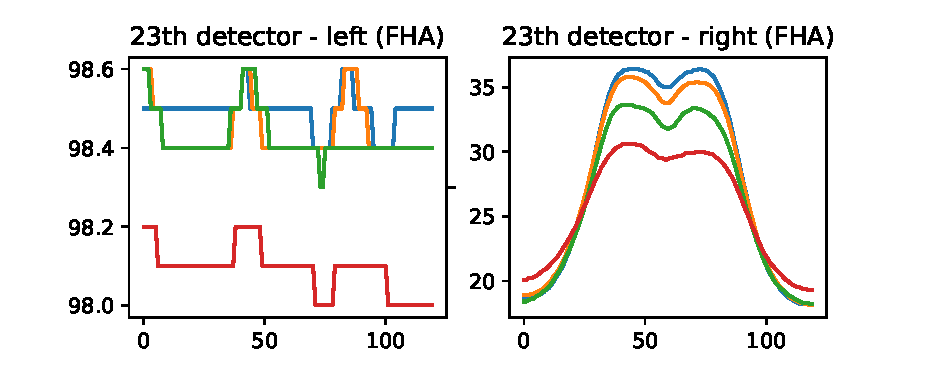
\includegraphics[width = \textwidth]{figures/sample.eps}}
    {}

\section{Features engineering}
The combination of the 5 features for every detectors and the 2 sides give a total of 50 features. To avoid a too high computation time on redundant features some of them are going to be selected. To select them a wrapper methods is going to be used with the selected classification algorithm, a random forest classifier. 

Before selecting the features the training set is going to be divided into 5 equals part, 4 of them are going to be used as training and 1 for testing. Then another one is used as testing etc. .

According to the size of the data set, the training of the model should not be too long, so rather high number of features can be selected. That is way a backward model has been preferred. The same argument apply for the choice of a wrapper methods rather than a filter approach. 

For the selection of feature a backward selection is performed, using trying to maximise the following.

  $f(Y)=\frac{1}{N} \sum_{k=1}^{N} W_{k},$ where $W_{k}\left\{\begin{array}{c}1 \text { if sample } Y_{k} \text { bewertung is correct } \\ 0.7 \text { if sample } Y_{k} \text { 'kurzbewertung is correct } \\ 0 \text { otherwise }\end{array}\right.$
  
In figure \ref{fig:Nfeature} features are selected, the relation between time of execution, performance and number of selected features is shown. It was expected that performance would have decrease with a lower number of features but it did not. An explanation could be the over-representation of some features having the same cause.

Same with the training time. But as the training time is rather low the time it took depend on the availability of power of the computer and might be bias. 
As the ratio performance/ time seems to be the best around 15 features, 15 are going to be selected, so a backward selection might not have been the best choice after all. 



\createfigure[h]
  {}
    {Selection of features}
    {\label{fig:Nfeature}}
    {\includegraphics[width = 0.9\textwidth]{figures/Nfeature.eps}}
    {}


Then a random forest model is design with the selected features. Then the performance of the model is compute as the value of the function with predicted and actual value of the test data set.

\section{Classification}
The same random forest algorithm is used. It is trained with the best performing train data set. The random forest has been chosen as it is better than a normal tree, has low risk of over fitting and allow the full usage of the computation power ( easy implementation of parallel computing ).


\section{Results}
\createtable[h]
{Title1} 
{Results}
{\label{tab:Results}} 
{\begin{tabular}{|c|l|c|c|c|c|c|c|c|c|c|c|c|}
\cline{3-13}
\multicolumn{2}{c|}{\multirow{2}{*}{}} &\multicolumn{11}{c|}{Predicted}\\ \cline{3-13}
\multicolumn{2}{c|}{} & E & F & Z & ZD & EH & EHWB & FHA & FHF & FHR & FHRB & FHRD\\\hline
\multirow{11}{*}{\begin{sideways}Real\end{sideways}} & E & 16 & 1 & 0 & 0 & 0 & 0 & 0 & 0 & 0 & 0 & 0\\  \cline{2-13}
& F & 0 & 142 & 4 & 0 & 0 & 0 & 0 & 0 & 0 & 0 & 0\\  \cline{2-13}
& Z & 2 & 0 & 9 & 0 & 0 & 0 & 0 & 0 & 0 & 0 & 0\\  \cline{2-13}
& ZD & 0 & 0 & 0 & 9 & 0 & 2 & 0 & 0 & 0 & 0 & 0\\  \cline{2-13}
& EH & 0 & 0 & 0 & 0 & 0 & 0 & 0 & 1 & 0 & 0 & 0\\ \cline{2-13}
& EHWB & 0 & 0 & 0 & 0 & 0 & 16 & 0 & 0 & 0 & 0 & 0\\\cline{2-13}
& FHA & 0 & 0 & 0 & 0 & 0 & 0 & 135 & 0 & 0 & 0 & 0\\\cline{2-13}
& FHF & 0 & 0 & 0 & 2 & 0 & 0 & 0 & 2 & 0 & 0 & 0\\  \cline{2-13}
& FHR & 0 & 0 & 0 & 1 & 0 & 0 & 0 & 0 & 0 & 0 & 0\\  \cline{2-13}
& FHRB & 0 & 0 & 0 & 1 & 0 & 0 & 0 & 0 & 0 & 0 & 0\\ \cline{2-13}
& FHRD & 0 & 0 & 0 & 0 & 0 & 0 & 0 & 0 & 0 & 0 & 5\\ \hline
\end{tabular}}
{}


\section{Conclusion} 

As the table \ref{tab:Results} show, there is really few miss classifications on short bewertung. As it is rather low, a two step classification (short than long) is not needed. The results are pretty good, maybe too much. The algorithm have a performance of 0.96, which is really good. There is some miss classification but mainly with 'Z' type, one could assume that 'Z' type will still be analysed in the future by expert. Concerning long bewertung the FHA which is the most represented category has not been miss classified. An explanation could be that as it is the most represented ( by far), they have been way more training to detect this type. Where the other have been more miss classified, the opposite argument apply. As they are under represented it is difficult for the algorithm to really determine a pattern. 


%\input{sections/Q1}
%\input{sections/Q2}


%%%%%%%%%%%%%%%%%%%%%%%%%%%%%%%%%%%%%%%%%%%%%%%%%%%%%%%%%%%%%%%%%%%%%%
%% Bibliography
%%   Leave this as is, and add you own entries to my.bib
%%   Many references are already defined in _latexfiles/bibs/all-eng.bib
%%   Refer to the BibTeX/LaTeX tutorial for adding new entries
%%   to the IVT BibTeX database
%\bibliography{_mybib}
%\bibliography{_latexfiles/bibs/all-eng,my}
%%%%%%%%%%%%%%%%%%%%%%%%%%%%%%%%%%%%%%%%%%%%%%%%%%%%%%%%%%%%%%%%%%%%%%

%%%%%%%%%%%%%%%%%%%%%%%%%%%%%%%%%%%%%%%%%%%%%%%%%%%%%%%%%%%%%%%%%%%%%%
%% Appendices
%%   Usually they would start on a separate page
%%%%%%%%%%%%%%%%%%%%%%%%%%%%%%%%%%%%%%%%%%%%%%%%%%%%%%%%%%%%%%%%%%%%%%

\clearpage

\end{document}

%%%%%%%%%%%%%%%%%%%%%%%%%%%%%%%%%%%%%%%%%%%%%%%%%%%%%%%%%%%%%%%%%%%%%%
%%%%%%%%%%%%%%%%%%%%%%%%%%%%%%%%%%%%%%%%%%%%%%%%%%%%%%%%%%%%%%%%%%%%%%
%%
%% END OF DOCUMENT
%%
%%%%%%%%%%%%%%%%%%%%%%%%%%%%%%%%%%%%%%%%%%%%%%%%%%%%%%%%%%%%%%%%%%%%%%
%%%%%%%%%%%%%%%%%%%%%%%%%%%%%%%%%%%%%%%%%%%%%%%%%%%%%%%%%%%%%%%%%%%%%%